\chapter{Consensus Algorithms Exercise 1}
\assignment{
  \textbf{Exercise 1} \\
  Let the graphs $G_1$, $G_2$, and $G_3$ be given as shown in Figure \ref{fig:consensus1}.
  \begin{enumerate}
  \item Derive the graphs $G_1 = (V_1, E_1)$, $G_2 = (V_2, E_2)$, and $G_3 = (V_3, E_3)$.
  \item Derive the Laplacian matrices of the graphs.
  \item Let $G_1$, $G_2$, and $G_3$ be the topology of a network of agents with integrator dynamics and consensus
    protocol
    \begin{equation}
      u_i = \sum_{j\in N_i} \left( x_j - x_i \right)
      \label{eq:coneqdyn1}
    \end{equation}
    Will the agents reach consensus, and if so, what type of consensus
    (consensus/average-consensus/min-consensus/max-consensus)?
  \end{enumerate}
  
  \begin{figure}[H]
    \centering
    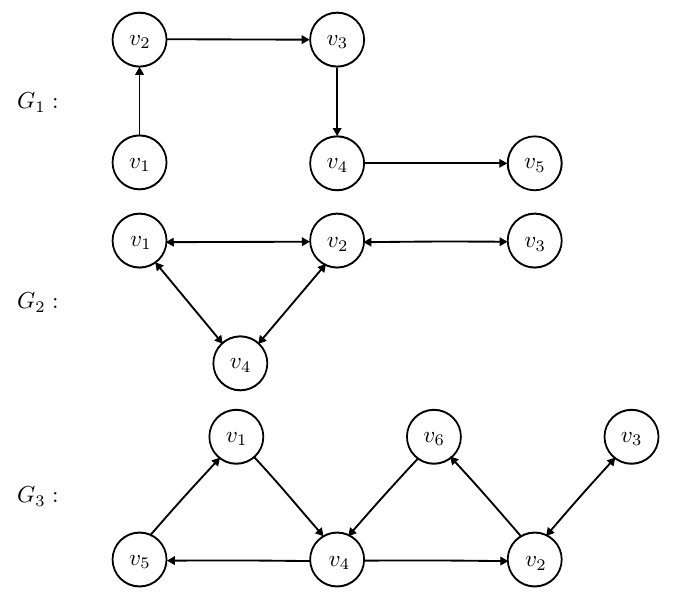
\includegraphics[width=0.8\textwidth]{consensus_fig1.png}
    \caption{Illustration of a dynamic graph.}
    \label{fig:consensus1}
  \end{figure}
}

\textbf{Derive the graphs:}           \\
\begin{equation}
  \begin{split}
    G_1 & = \{ v_1, e_1 \}            \\
    V_1 & = \{ v_1,v_2,v_3,v_4,v_5 \} \\
    E_1 & = \{ (v_1,v_2),(v_2,v_3),(v_3,v_4),(v_4,v_5) \}
  \end{split}
\end{equation}
\begin{equation}
L_1 = 
  \begin{bmatrix}
    0   & 0  & 0  & 0  & 0            \\
    -1  & 1  & 0  & 0  & 0            \\
    0   & -1 & 1  & 0  & 0            \\
    0   & 0  & 0  & -1 & 1 
  \end{bmatrix}
\end{equation}
\begin{equation}
  \begin{split}
    G_2 & = \{ V_2,E_2 \}             \\
    V_2 & = \{ v_1,\ldots,v_5 \}      \\
    E_2 & = \{ v_{12}, v_{21}, v_{14}, v_{41}, v_{42}, v_{24}, v_{23}, v_{32} \}
  \end{split}
\end{equation}
\begin{equation}
  L_2 = 
  \begin{bmatrix}
    2   & -1 & 0  & -1                \\
    -1  & 3  & -1 & -1                \\
    0   & -1 & 1  & 0                 \\
    -1  & -1 & 0  & 2
  \end{bmatrix}
\end{equation}
\begin{equation}
  \begin{split}
    G_3 & = \{ V_3,E_3 \}             \\
    V_3 & = \{ v_1,\ldots,v_6 \}      \\
    E_3 & = \{ v_{51}, v_{14}, v_{45}, v_{64},v_{42},v_{26},v_{32},v_{23} \}
  \end{split}
\end{equation}
\begin{equation}
  L_3 = 
  \begin{bmatrix}
    1   & 0  & 0  & 0  & -1 & 0       \\
    0   & 2  & -1 & -1 & 0  & 0       \\
    0   & -1 & 1  & 0  & 0  & 0       \\
    -1  & 0  & 0  & 2  & 0  & -1      \\
    0   & 0  & 0  & -1 & 1  & 0       \\
    0   & -1 & 0  & 0  & 0  & 1
  \end{bmatrix}
\end{equation}

Balanced => strongly connected
Strongly connected =!> Balanced (sometimes it does, not always)
Remark that any undirected graph is balanced.

Average-consensus is achieved in G2 and G3, in G1 the group decision is the value in vertice 1

\assignment{
  \textbf{Exercise 2} \\
  Consider the two graphs $G_1 = (V_1, E_1)$ and $G_2 = (V_2, E_2)$, where \\
  $V_1 = \left\{v_1, v_2, v_3, v_4\right\},\, V_2 = \left\{v_1, v_2, v_3 , v_4 , v_5, v_6 \right\},$ \\
  $E_1 = \left\{e_{12}, e_{21} , e_{23}, e_{32}, e_{24}, e_{42}, e_{34}, e_{43}, e_{14}, e_{41} \right\},$ \\
  $E_2 = \left\{e_{12} , e_{23} , e_{31}, e_{14} , e_{41} , e_{43}, e_{36} , e_{65} , e_{54} \right\}.$ \\
  \begin{enumerate}
  \item Derive the convergence rate of the disagreement of the two dynamic networks with topology G1 and G2 and agents
    governed by integrator dynamics consensus protocol in equation \eqref{eq:coneqdyn1}.
  \item Simulate the dynamic networks and compare the simulated results with the convergence bound.
  \end{enumerate}
}

\begin{equation}
  \begin{split}
    G_1 & = \{ V_1,E_1 \}, G_2 = \{ V_2,E_2 \}                                          \\
    V_1 & = \{ v_1,\ldots,v_4 \}, V_2 = \{ v_1,\ldots,v_6 \}                            \\
    E_1 & = \{ e_{12},e_{21},e_{23},e_{32},e_{24},e_{42},e_{34},e_{43},e_{14},e_{42} \} \\
    E_2 & = \{e_{12},e_{23},e_{31},e_{14},e_{41},e_{43},e_{36},e_{65},e_{54}\}
  \end{split}
\end{equation}
\begin{equation}
  L_1 = 
  \begin{bmatrix}
    2   & -1 & 0  & -1                                                                  \\
    -1  & 3  & -1 & -1                                                                  \\
    0   & -1 & 2  & -1                                                                  \\
    -1  & -1 & -1 & 3
  \end{bmatrix},\quad
  L_2
  \begin{bmatrix}
    2   & 0  & -1 & -1 & 0  & 0                                                         \\
    -1  & 1  & 0  & 0  & 0  & 0                                                         \\
    0   & -1 & 2  & -1 & 0  & 0                                                         \\
    -1  & 0  & 0  & 2  & -1 & 0                                                         \\
    0   & 0  & 0  & 0  & 1  & -1                                                        \\
    0   & 0  & -1 & 0  & 0  & 1
  \end{bmatrix}
\end{equation}
A laplacian can be converted to a laplacian for the mirror graph by:
\begin{equation}
  \bar{L}_1 = \left( L_1 + L_1\transp \right)\frac{1}{2}
\end{equation}

\begin{equation}
  \bar{L}_1 =
  \begin{bmatrix}
    4 & -2 & 0 & -2 \\
    -2 & 6 & -2 & -2 \\
    0 & -2 & 4 & -2 \\
    -2 & -2 & -2 & 6
  \end{bmatrix}
  \frac{1}{2} \Rightarrow L_1 = \bar{L}_1 \Rightarrow \lambda_2 = 2
\end{equation}

\begin{equation}
  \bar{L}_2 =
  \begin{bmatrix}
    4 & -1 & -1 & -2 & 0 & 0 \\
    -1 & 2 & -1 & 0 & 0 & 0 \\
    -1 & -1 4 & -1 & 0 & -1 \\
    -2 & 0 & -1 & 4 & -1 & 0 \\
    0 & 0 & 0 & -1 & 2 & -1 \\
    0 & 0 & -1 & 0 & -1 & 2
  \end{bmatrix}
  \frac{1}{2} \Rightarrow \lambda_2 = 0.6
\end{equation}

\assignment{
  \textbf{Exercise 3} \\
  The graph $G = (V, E)$ with vertices $V = \{v_1, v_2, v_3, v_4 , v_5 \}$ and edges $E = \{e_{12} , e_{23}, e_{34} ,
  e_{45} \}$ reaches consensus with consensus protocol \eqref{eq:coneqdyn1}. Modify the consensus algorithm such that the network
  converges to
  \begin{equation}
    \begin{bmatrix}
      x_1 - x_2 \\
      x_2 - x_3 \\
      x_3 - x_4 \\
      x_4 - x_5
    \end{bmatrix}
    =
    \begin{bmatrix}
      1 \\
      3 \\
      9 \\
      2
    \end{bmatrix}
  \end{equation}
}

\assignment{
  \textbf{Exercise 4} \\
 Add a virtual agent to the dynamic network in Figure \ref{fig:consensus2} such that the state of every agent follows
 the constant reference of the virtual agent.
 \begin{figure}[H]
   \centering
   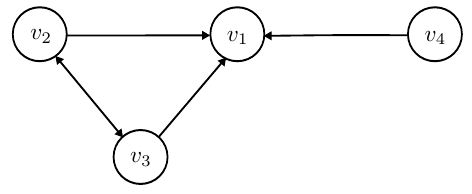
\includegraphics[width=0.5\textwidth]{consensus_fig2.png}
   \caption{Illustration of a dynamic graph}
   \label{fig:consensus2}
 \end{figure}

}
